\documentclass{article}
\usepackage[utf8]{inputenc}
\usepackage{graphicx}
\usepackage[left=2cm, right=2cm, top=2cm]{geometry}
\usepackage{etoolbox}
\usepackage{caption}
\usepackage[margin=1in]{geometry}
\newcommand\tab[1][1cm]{\hspace*{#1}}
\usepackage[export]{adjustbox}

\title{Symbiotic organisms search algorithm for the blood assignment problem}
\author{Prinolan Govender\textsuperscript{1}, Absalom Ezugwu \textsuperscript{2}}
\date{\textsuperscript{1}School of Mathematics, Statistics, and Computer Science, University of Kwazulu-Natal, Private Bag Box X54001, Durban 4000, South Africa}

\begin{document}

\maketitle
\begin{abstract}
  \textbf{Abstract}: The demand for blood transfusion is a real world problem which is needed for various medical emergencies. The blood assignment problem was introduced to address this problem. The blood assignment problems formulation stretches from managing critical blood shortage levels, blood unit expiration, to blood compatibility between donor blood and patients. Another contributing factor to the blood assignment problem, lies in the blood bank having to import additional blood units from external sources when supply cannot meet the demand. These challenges have serious consequences especially in the case where the demand for blood is very high. Taking these factors into consideration, the following study implements a metaheuristic hybrid algorithm that combines symbiotic organisms search algorithm with blood assignment policy in relation to the blood banks of South Africa. The aim of this study is to minimize blood product wastage with regards to expiration and importation, whilst maximizing product delivery to patients in need. In addition, this study also implements a unique way in generating randomized datasets based on social events relating to South Africa public holidays. The computational results indicate that the symbiotic organism search performed well in minimizing blood importation, and experienced no form of expiration throughout the time period.
  \\
  \\
\textit{Keywords: Symbiotic organism search algorithm, blood assignment, metaheuristic, blood demand, blood supply}

\end{abstract}

\section{Introduction}
Human blood inventory management is categorized by a string of influences which contributes to its efficiency and can complicate as time progresses [1]. In the past years, many aspects of blood management have been introduced and scrutinized in order to implement dynamic policies and strategies that would optimize the management process. Blood is a perishable commodity with unique medical value to humans [2]. The unique composition of blood enables the substance to carry vital components through-out the human body, and also disposes of waste material. Blood consists of four (4) major components namely red blood cells (RBC), white blood cells (WBC), and blood platelets, all of which is immersed in a matrix of plasma. This paper focuses on the combination of all these components which is referred to as whole blood (WB) units. The WB units can voluntarily be donated to blood centres, which initiate the process of blood screening and storing of WB units in appropriate conditions. In accordance to the blood system, often referred to as the ABO system [3], there exist 4 blood groups in humans namely A, B, AB and O. Each of these blood groups have a Rhesus value (Rh) which can either be positive (+) or negative (-), which therefore results in 8 different blood types. Blood compatibility plays a vital role in blood management and distribution of such units, cases have risen were patients received incompatible blood types which resulted in blood clumping (also referred to as agglutination), which can be life threatening. \\
\\
The blood assignment problem (BAP) can simply be defined as an optimization process which efficiently assigns a supply of WB units to the daily demand of these units. The BAP has a plethora of underlying external components which contributes to the complexity of the problem. However, the main issue relates to the demand for WB units. Demand can be separated into two scenarios, the first type of demand relates to an expected need for WB units which can be arranged a few days prior to using it, a typical example for such a scenario is the everyday surgeries that occurs in the hospitals. It is the second form of demand which complicates blood management, this scenario relates to an unforeseen demand for WB units and this type of demand pertains to patients who experience sudden onsets of trauma which requires immediate need for medical attention and WB units. Taking these scenarios into account, and other contributing factors, it is therefore possible to establish an objective for the BAP, which is to minimize the combination of both expiration and additional importation (from external sources) faced by the blood bank. By minimizing the objective function, the BAP would be deemed as efficient.
\\
\\
In this paper, the possibility of improving the recently proposed symbiotic organisms search (SOS) algorithm with an efficient blood assignment model to solve the BAP is investigated in this paper. The symbiotic organisms search algorithm was first introduced in [15] to solve complex structural engineering design optimization problems. The algorithm is inspired by the symbiotic relationships strategies, which exist among organisms in the ecosystem. SOS is capable of providing efficient and robust approach in exploiting and exploring large search space, more so, it has been employed to optimize a number of combinatorial optimization problems and have proved to be an efficient performer in that aspect [16], [17], [18], [19]. Therefore, the potential of SOS in finding good quality solutions to most real-world optimization problem makes it attractive for further investigation. In addition, SOS has not gained wide recognition in solving inventory problems and it has not been attempted on the blood assignment problem. This can be considered as the main motivation for introducing the algorithm to solve such a complex discrete optimization problem like the BAP.
\\
\\
This paper explores the possible hybridization of the symbiotic organism search (SOS) algorithm coupled with a robust blood bank management policy. Due to confidentiality issues, the following study could not use any real-world data, therefore datasets were randomly generated. In existing related literatures, datasets were also randomly generated using a set of percentage bounds across a finite time period. However, this paper explores a different method or policy for generating stochastic datasets, by incorporating statistics adapted from South Africa social trends in order to form these percentage bounds. This technique is further discussed in the later section of this paper.  The policy also takes into account other contributing factors which could affect the management of blood. These factors include: blood compatibility, the first-in first-out (FIFO) issuing system, expiring WB units and importing additional WB units from external sources.
\\
\\
In the last decade, a number of heuristic based algorithmic strategies were proposed in the quest for finding near-optimum solutions to the inventory blood assignment problem, among these algorithms include Hill climbing (HC) [37, 38], Simulated annealing (SA) [37, 38], Genetic algorithm (GA) [3, 36, 38], Tabu search (TS) [39], Particle swarm optimization (PSO) [12], Greedy Randomized Adaptive Search Procedure (GRASP) [13]. All the algorithms listed here draw their inspiration from nature, through the observation of physical processes that occur in nature. They are implemented by mimicking different natural systems and processes using mathematical models and algorithms. However, aside GA and PSO none of the aforementioned heuristics have proven track record of finding good near-optimum solution to complex real-world problems in the domain of combinatorial optimization.
\\
\\
The rest of the paper is organized as follows: section 2 reviews previous work pertaining to the BAP, section 3 illustrates the methodology used in formulating and solving the BAP proposed in this paper, Section 4 presents experimental settings, dataset configurations, results and discussions. Finally concluding remarks and future work are discussed in section 5.


\section{Related Work}
Blood transfusion is a daily activity which occurs in most hospitals around the world. The study of blood transfusion dates back to the early 1900’s when the discovery of the ABO blood grouping system was introduced [3]. This system reduced the negative side effects faced by patients who commonly experienced blood clumping.  In [4] a linear model for blood management was introduced, which merged a dynamic environment for blood products entering and leaving the management system. The model introduced by [5] also took into account blood compatibility and identified a solution when the demand equated to the supply for a day. Bas [5] analysed another aspect of the blood banking system which focused on the donating process of blood. The study looked into donors, collection and screening of acquired blood units as well as finding a way of supplying an adequate supply of blood units to transfusion centres. The management of blood is a diverse topic with many different areas of consideration.
\\
\\
In recent years, some of the research conducted in [2], [6], and [7], were in relation to the BAP, and followed the same assignment patterns in terms of proposing an optimization models for the blood assignment problem. Each of the studies implemented the usage of a multiple knapsack model that enabled the cross-matching of blood between compatible types. The following table illustrates the compatibility between blood types. Table 1 Represents the compatibility between blood types while “YES” implies that the blood types are compatible, and “NO” implies that the blood types are not compatible.
\begin {center}
Table 1: {Representation of blood compatibility }
\break
\end {center}

    
\begin{center}
\begin {tabular}{|c|c|c|c|c|c|c|c|c|}
\hline

Blood types& $A^+$&$A^-$&$B^+$& $B^-$& $AB^+$& $AB^-$&  $O^+$& $O^-$ \\ [0.5ex]
\hline
 $A^+$&YES&YES&NO&NO&NO&NO&YES&YES\\
 $A^-$&NO&YES&NO&NO&NO&NO&NO&YES\\
 $B^+$&NO&NO&YES&YES&NO&NO&YES&YES\\
$B^-$&NO&NO&NO&YES&NO&NO&NO&YES\\
$AB^+$&YES&YES&YES&YES&YES&YES&YES&YES\\
$AB^-$&NO&YES&NO&YES&NO&YES&NO&YES\\
$O^+$&NO&NO&NO&NO&NO&NO&YES&YES\\
$O^+$&NO&NO&NO&NO&NO&NO&NO&YES\\
\hline

\end {tabular}

\end {center}
Including the multiple knapsack model, the studies also implemented the bottom-up technique to utilise additional units from compatible blood types. The difference between studies [2], [6], and [7], lies behind the metaheuristic algorithms that was used to work the BAP. In [6], an extensive study which utilised different adaptations of Genetic Algorithms (GA) such as Adaptive Genetic Algorithm (AGA), Simulated Annealing Genetic Algorithm (SAGA), Adaptive Simulated Annealing Genetic Algorithm (ASAGA) as well as Hill Climbing (HC) Algorithm were considered. The results showed that the HC implementation yielded the best results with the other implementations also producing satisfactory outcomes. In [2], the Particle swarm optimization (PSO) algorithm was used to solve the BAP, with results showing no form of wastage and very low importation levels. The study conducted in [7] utilised 2 local search algorithms namely Dynamic programming (DP) and GRASP, the study in [7] also implemented a system which introduced the previous days remaining blood units to the current days’ supply. The results achieved by their proposed methods show that GRASP imported blood types O+ and O- quite heavily for the first 50 days, before levelling out, whilst DP proved to be more efficient when demand exceeded supply.
\\
\\
The current study incorporates certain components used in previous literature. A notable gap from previous related literatures is the lack of availability of datasets and the manner in which the employed stochastic datasets were generated and used for testing the existing implementations. Most studies simply introduce percentage bounds to generate levels for supply and demand. The following study tries to reduce the randomness when generating such values by incorporating South African social trends monthly statistics, which is achieved by including monthly public holidays and educational institution terms, in an attempt to generate values which, mimic real-life monthly demands for WB units. 
\\
\\
South Africa is often referred to as the “rainbow nation” due to its variety of culture and race. Race refers to the ethnicity of an individual, there exists four common races in South Africa, Black Africans, White, Indian, and Coloured, with approximately 41 million citizens currently living in South Africa [8]. The Pie chart shown in Fig. 1 indicates the current percentage of races within the population.


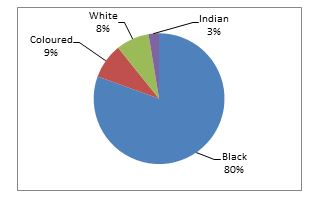
\includegraphics[width=0.5\textwidth, center]{Images/PieNew.JPG}
\begin {center}
Fig 1: The 2018 race group proportions in South Africa adapted from [9]
\end {center}
\\
\\
Figure 1 indicates that the current percentage of Black South African citizens is 80.6\%, Coloured is 8.7\%, White citizens are 8.2\% and finally the Indian population is 2.6\%. The proportion of race groups in South Africa plays a vital role with regards to HIV and AIDS. The disease is an acquired virus which attacks an individual’s immune system [10] which currently has no cure. In South Africa an estimated 7 million people are currently affected with HIV, with an annual death toll of approximately 180 000 people and an estimated 64\% of the infected individuals being of the Black racial group [8]. Therefore, this further justifies the screening process of blood for any blood related diseases and pathogen before it reaches the patient in need. Due to the variety of culture in South Africa, the country also experiences a number of different public holidays. These holidays are derived from a variety of events, some of which are issued to honour the past of South African history (especially related to the Apartheid era), whilst others are culturally based. In addition to public holidays, educational facilities such as schools and tertiary institutes take mid-term breaks. The importance of these dates relates to the social behaviour aspect that will be represented in the current study of the BAP. In theory, individuals indulge in more dangerous activities during months with more breaks and public holidays, therefore leading to an increase in demand of blood and blood products (see further discussion in Section 3). Table 2 illustrates the proportion of blood types found in the South African population [2].
\begin {center}
Table 2: {Illustrates the proportion of blood types found in the South African Population adapted from [12] }

\end {center}
\begin{center}
\begin {tabular}{|c|c|c|c|c|c|c|c|c|}
\hline

Blood types& $A^+$&$A^-$&$B^+$& $B^-$& $AB^+$& $AB^-$&  $O^+$& $O^-$ \\ [0.5ex]
\hline

 $Proportion(\%)$&32&5&12&2&3&1&39&6\\
 
\hline

\end {tabular}

\end {center}

\section{Methodology}
The demand and supply for WB units follow a stochastic trend. In an ideal day, the supply for each blood type would be commensurate to the level of demand and this would result in no form of remainder that would invites possible expiry, or any importation that would increase the costs incurred by the blood bank. The following section presents a more in-depth understanding of the proposed hybridization process between the SOS and blood bank management policy.

\subsection{Problem Formulation}
Every day the demand for WB units must be met. If the daily supply is greater than or equal to the daily demand, then the supply is distributed accordingly and the demand is considered as satisfied. However, if the daily demand exceeds supply, this then initiates other processes to that would meet the desired level for demand. First, the blood bank must check for compatible blood types and use only the remaining units from the blood groups (each blood type is expected to fulfil their respective demand first). If pulling from additional blood units still has not satisfied the demand, then the blood bank must import additional units from external sources in order to satisfy the request. Newer blood units often accumulate as a result of voluntary donations, once blood screening has taken place only then are WB units added to storage. To reduce expiry, the WB units enter a queuing system, which can also be referred to as the First-in-first-out (FIFO) system, which allows for older WB units to be used first, thus reducing the possibility of expiry. Any units that have exceeded their lifespan will be discarded from the blood bank. It must be noted that the act of importing and discarding WB units incur additional costs for the blood bank. Overall the BAP can be summarized into 4 major components as follows:
\\
\\
•	\textbf{Supply}: this relates to the current stock of WB units on hand at the beginning of the day. The previous day’s remainder is added to the daily influx of donations to equate to a final supply value.\\
•	\textbf{Demand}: this relates to both unplanned and planned requests for the need of WB units.\\
•	\textbf{Importation}: this relates an instance were, additional WB units are imported when the demand levels exceeds the supply levels for a day\\
•	\textbf{Expiring}: WB units that have exceeded their shelf life are discarded in an appropriate manner.\\
\\
Due to the plethora of external factors which encumber the BAP, certain assumptions were made in this paper in order to formulate the required mathematical model that would be sufficient for the problem at hand. These assumptions are as follows:\\
\\
•	The blood bank has an infinite supply of capital, and storage space. The external sources (for importing WB units) also have a limitless supply.\\
•	The time frame will be conducted over 365 days, with day 1 receiving no carryover of WB units from the previous day.\\
•	Validity of blood will be set at 30 days.\\
•	All blood types will first fulfil requests associated with their blood types, from there the remainder from each blood group can contribute to other compatible blood types.\\
\\
\subsection{Objective Function}
The objective function for the BAP relates to minimizing expiration and importation of WB units within a blood bank. As such, the following equations represent the objective function used in this study.
Let
\\
\\
\textit{I}: Represent the amount of importation	\\	                   
\textit{E}: Represent the amount of expiration	\\	                    
\textit{d}: Represent the day\\
\\
Min: \sum{_{d=1}^n}(I{_{Total}} + E{_{Total}}){_d}\tab[12,7cm] (1)\\
Where:\\
1$\leq$ d $\leq$ 365\\
I{_{Total}}={I{_A}^+}(d) + {I{_A}^-}(d) + {I{_B}^+}(d) + {I{_B}^-}(d)+ {I{_AB}^+}(d) + {I{_AB}^-}(d) + {I{_O}^+}(d) + {I{_O}^-}(d)\tab[4cm](2)\\
E{_{Total}}={E{_A}^+}(d) + {E{_A}^-}(d) + {E{_B}^+}(d) + {E{_B}^-}(d)+ {E{_AB}^+}(d) + {E{_AB}^-}(d) + {E{_O}^+}(d) + {E{_O}^-}(d)\tab[2,5cm] (3)\\

By minimizing the objective function stated in eq. 1, the BAP is successfully optimized\\
\subsection{Generating Demand and Supply}
Due to confidentiality issues, it was not possible to use real-world datasets in this study. Instead a randomly generating datasets which utilises South African social trends based on monthly statistics. By incorporating monthly holidays as well as terms from educational institutions, it is theoretically possible to create unique percentage bounds and allocate them to each month, which in turn reduces randomness when generating dataset values. The ideology behind this method is to show that the demand for blood has trends associated with a specific month, for example demand would be expected to have a higher value in a month like December due to many people being off from work, school and other institutions, as well as the rise of dangerous events such as drinking and driving and criminal activities. Reports have previously indicated that levels of drunk driving increases during the Easter period [11], thus blood banks tend to stock-pile blood products for precautionary measures during this public holidays. In terms of generating percentage bounds for supply, there was no significant events that occurred during a standard South African year, therefore the percentage bounds will be set between 25-75\%. Table 3 represents the starting month and ending month of most educational institutions in South Africa [12]. Table 4 represents the public holidays in South Africa within a year and Table 5 illustrates the percentage bounded ranges used for generating demand.
\begin {center}
Table 3: {Starting month and ending month of most educational institutions in South Africa.}

\end {center}
\begin{center}
\begin {tabular}{|c|c|c|}
\hline

Education institutions terms& Start Month&End Month \\ [0.5ex]
\hline

 $1$&January&March\\
  $2$&April&June\\
   $3$&July&September\\
    $4$&October&December\\
\hline

\end {tabular}

\end {center}

\begin {center}
Table 4: {: Public holidays in South Africa within a year}

\end {center}
\begin{center}
\begin {tabular}{|c|c|}
\hline

Date& Public Holiday \\ [0.5ex]
\hline

 $1 January$&New year’s day\\
  $21 March$&Human Rights day\\
   $14 April$&Good Friday\\
    $17 April$&Family day\\
     $27 April$&Freedom day\\
      $1 May$&Workers day\\
       $16 June$&Youth day\\
        $9 August$&Woman’s day\\
         $24 September$&Heritage day\\
          $16 December$&Day of recognition\\
            $25 December$&Christmas day\\
              $26 December$&Boxing day\\
\hline

\end {tabular}

\end {center}
\begin{center}
    Using tables 3 and 4 from above, it is now possible to link each month with a unique percentage bound
\end{center}



\begin {center}
Table 5:  {Percentage bounded ranges used for generating demand.}

\end {center}
\begin{center}
\begin {tabular}{|c|c|}
\hline

Month&Percentage bounds  \\ [0.5ex]
\hline

 $January$&35-85\\
  $February&25-50\\
   $March&25-75\\
    $April$&65-90\\
     $May&25-75\\
      $June&35-85\\
       $July&65-90\\
        $August$&25-75\\
         $September$&10-50\\
          $October&25-75\\
            $November&25-75\\
              $December&65-90\\
\hline

\end {tabular}

\end {center}
Using the percentage bounds in table 5, it is now possible to generate demand, as well as supply using eq 2.\\
\break
Therefore, if we denote following as:\\
A: Represent the initial volume in a blood bank    \\        
d: Represent a day	\\			
m: Represent a month\\			
b: Represent a blood type 	\\		
$B{_u}$: Represents the Upper percentage bound\\	
$B{_l}$: Represent the lower percentage bound\\	
rng: Represents a random generator\\
\break
$Supply{_b}\tab[0,5]or Demand{_b} = A . (rng(B{_u}-B{_l}){_m})$\tab[10cm](4)\\
\break
From eq 4, the supply or demand is generated by randomly selecting a percent between the upper and lower bounds depending on the month the system is currently in (this is established in accordance to the current day). This is then multiplied by the initial volume in the blood bank to generates a value for supply or demand. The process for generating supply has an additional step, which involves adding the previous days’ remainder (as long as the remainder is greater than 0). However, if the system is in the first day, then remainder is taken as 0. Therefore, using the percentage bounds in Table 5 above, it is now possible to generate demand, as well as supply using eq 4.\\

\subsection{Expiring Blood Units}
WB units are deemed as a perishable commodity due to its limited shelf-life. This implies that a WB unit will be destroyed if it is not being used or distributed within 30 days of its first entry into the blood banking system. The heuristic presented in Algorithm 1 illustrates the conditions that must be satisfied in order for expiry to occur. It is unlikely for expiry to occur when the daily demand and supply have similar levels or the daily demand exceeds the daily supply over a period of days. However, if this phenomenon occurs then it is unlikely for a unit of blood to be on the shelf for 30 days.\\
\break

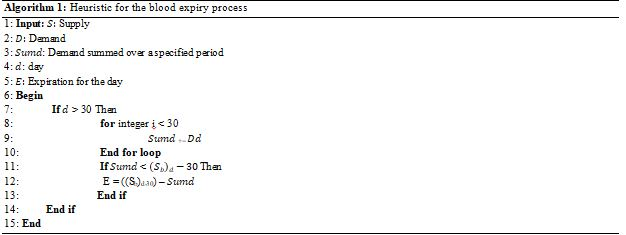
\includegraphics[width=0.7\textwidth, center]{Images/Alg1.JPG}
\begin {center}
The above heuristic presented as Algorithm 1, only occurs after day 30, due to WB units having a lifespan of 30 days. Therefore, it’s impossible to have units expiring before this time, this also allows the implemented system to be more efficient. In Algorithm 1 above, Sb denotes the supply of each blood type
\end {center}
\subsection{Bottom-up Technique}
When the WB units on hand cannot meet the demand for a day, additional WB units from other blood types that are compatible are used. Each blood type must first fulfil their corresponding requests for the day before they can be distributed to other compatible blood types. The bottom-up technique used in [2] [6] and [7] relates to a system which utilises blood from other compatible blood types in order to fulfil the days’ requests only when demand exceeds supply. Therefore, it can be established that the remainder from a day is then split according to the number of possible compatible types. By implementing this technique, the blood bank will reduce importation of blood units, and utilises its resources more effectively. It is noteworthy to mention here that the current study did not consider the medical case were the patient’s specific blood type must be used. Table 6 represents the various blood types and the compatible blood types they can be matched with.\\
\break
\begin {center}
Table 6: {Blood types and their compatible blood types}

\end {center}
\begin{center}
\begin {tabular}{|c|c|c|}
\hline

Blood Types& Can distribute to&Splitting \\ [0.5ex]
\hline

 %$A{_+}$&A{_-}O{_+}O{_-}&Remainder of A{_+}\\
  $A{^+}$&$A{^-},O{^+},O{^-}$&$ $(Remainder A{^+})/3$\\
 $A{^-}$&$O{^-}$&$ $(Remainder A{^-})/1$\\
   $B{^+}$&$B{^-},O{^+},O{^-}$&$ $(Remainder B{^+})/3$\\
   $B{^-}$&$O{^-}$&$ $(Remainder B{^-})/1$\\
   $AB{^+}$&$A{^+},A{^-}, B{^+}, B{^-}, AB{^-},O{^+},O{^-}$&$ $(Remainder AB{^+})/7$\\
   $AB{^-}$&$A{^-},B{^-},O{^-}$&$ $(Remainder AB{^-})/3$\\
   $O{^+}$&$O{^-}$&$ $(Remainder O{^+})/1$\\
   $O{^-}$&N/A&$ $N/A$\\
\hline

\end {tabular}

\end {center}

The act of pulling blood is conducted in accordance with the order of blood proportions in South Africa (as shown in Table 2). The higher the proportion of a blood type, the chances of it being distributed first. For example, if the blood type A+ is to be pulled from additional units, it would first pull from O+ blood which has a proportion of 39\%, if the demand is still not satisfied, more blood units will be pulled from O- and finally if the demand still exceeds supply, more units will be pulled from A-. After conducting the bottom-up technique, if the demand still exceeds supply, then additional WB units is imported. This method of pulling from compatible blood units in this particular order is applicable to rarest of the blood types and the entire process aims at maximizing the storage of blood types which have the lowest proportion (have a higher rarity). More common blood types also have a higher percentage of resupply in the future.\\
\subsection{Solution Representation}
As mentioned previously, blood has eight (8) different types for humans, which we donate here as organisms. Using this information, it is possible to extrapolate a solution representation pattern for an individual organism within a population of ecosystem. The individual organisms are finite with 8 segments, and each segment is represented with a specific blood type capable of containing a value of type double. Fig. 2 depicts the individual organism used in the SOS algorithm with each segment representing an individual blood type and a specific numerical value.\\
\\
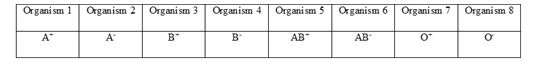
\includegraphics[width=0.7\textwidth, center]{Images/Solution.JPG}
\begin {center}
Fig 2:Solution representation for the BAP
\end {center}
\subsection{Symbiotic Organism Search Algorithm}
The SOS is an algorithm which emulates the interactive behaviour of creatures within nature [13], with a notable advantage of no specific parameter tuning which decreases time in order to achieve good results [14]. The SOS can be dissected into 3 main optimization phases namely mutualism, commensalism and parasitism, each of these phases tries to modify the chosen individual(s) with the hopes of obtaining a more improved solution. The individuals and their blood types are represented using the solution representation shown in Fig 2 above, the SOS subsequently employs the solution representation to solve the BAP with each SOS organisms representing human individual and the blood type being assigned a specific value. The three algorithm’s phases are modelled as follows: \\
\\
\textbf{Mutualism}: Organisms interact with each other in a way that benefits both parties. Let $X{_i}$  and $X{_j}$  represent 2 random individuals within a population, MV represent the Mutual Vector, $X{_{best}}$ represent the organism with the best advantage, and BF represent the benefit factor. The mutualism phase is presented using the following equations.
\\
\\
X{_{inew}} = X{_i} +rand(0,1) . ($X{_{best}}$ - MV . BF1)\tab[10cm] (5)\\
X{_{jnew}} = X{_j} +rand(0,1) . ($X{_{best}}$ - MV . BF2)\tab[9,97cm] (6)\\
\\
Where:
\\
$MV=(X{_i} + X{_j})/2\tab[14cm](7)$\\
\\
The value obtained from ($X{_{best}}$ – MV) tries to increase survival in the population, with all improved individuals replacing the original individuals. The values of the benefit factors BF1 and BF2 are determined randomly using equations 8 and 9.\\
\\
$BF1 = (1 + round(rand(0,1))), rand \in [0,1]\tab[10cm](8)$\\
$BF2 = (1 + round(rand(0,1))), rand \in [0,1]\tab[9,95cm](9)$
\\
\\
where round and rand are MATLAB function. The round function rounds up generated values to the nearest whole number and the rand function generates random number.
\\
\\
\textbf{Commensalism}: In this phase, the individual organism interacts with each other in a way that results in one organism benefiting without harming the other organism. Selection of two organisms is done randomly from the population, and have their fitness values evaluated, the fitter individual is labelled as X{_i} and the inferior individual is labelled as X{_j}.\\
\\
X{_{inew}} = X{_i} + rand(-1,1) . ($X{_{best}}$ - X{_j}\tab[10,7cm](10)\\
$X{_i}$ benefits from $X{_j}$ by means of $($X{_{best}}$ - X{_j})$\tab[9,5cm](11)\\
\\

\textbf{Parasitism}: In this phase, the organisms interact with each other in a way that benefits one organism (parasite) whilst harming the other organism (host). To evaluate a form of parasitism for the BAP, two individuals from a population are randomly selected, with each of its fitness values evaluated similar to the commensalism phase. Following the evaluation, the fitter individual is labelled as the parasite, and the inferior as the host. The parasite then swaps segments of its representation with the host only if the value (from the host) improves its original solution. The following algorithmic steps illustrates the parasitism procedure (Algorithm 2), which has been improved to make the SOS suitable for solving the BAP.\\
\\
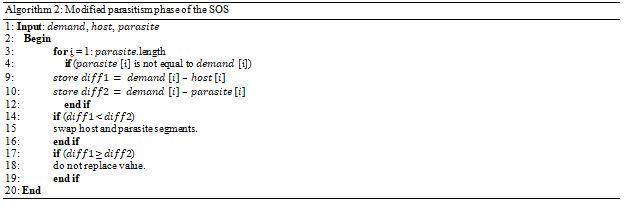
\includegraphics[width=0.8\textwidth, center]{Images/alg2.JPG}
\\
\\

Algorithm 2 illustrates the parasitism process conducted in this study of the BAP. The parasite analyses the host and swaps segments if the host contains a better value than itself. The values for both the host and parasite are matched against the demand for the day (per blood type) in order to deduce the better value. The algorithm 3 below represents the general implementation of the improved SOS algorithm. The improved SOS algorithm incorporates the three basic SOS algorithm’s phases discussed earlier to implement the BAP.\\
\\
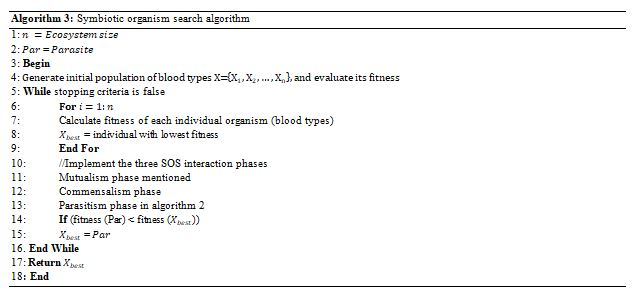
\includegraphics[width=0.8\textwidth, center]{Images/Alg3.JPG}
\\
\\
It is noteworthy to mention here that because the basic SOS algorithm was originally designed for continuous optimization problem and the BAP being a combinatorial optimization problem, a random permutation process of using a modulus function given by u=$⌊$x+k$⌋$ mod m was used to convert the solution x to an integer u, where, k and m$<$0 are integers.  

\section{Experimental Setting and Dataset Generation}
The SOS algorithm was implemented on Intel core i5 CPU with 2.5GHz and 4GB RAM and Windows 10.0 Operating system, while the implementation software is Java. For each data sets, the algorithm was run for 1000 number of iterations, using population size of 50 organisms. As it was mentioned previously that the current study faced confidentiality issues with dataset acquisitions, therefore the study resorted to generating datasets by means of incorporating fixed percentage bounds between the ranges of 25 to 75\%. This was used to generate both demand and supply. This study tries to minimize the randomness when generating demand values, by incorporating public holidays and schooling terms based on the South Africa vacation trends, referred here as South African generated values (SAGV). The ideology for introducing such factors lies behind social convention, as people are more prone to conducting dangerous activities such as drinking and driving or criminal activities during festive periods or during months with more public holidays. Therefore, using this logic, it can be interpreted that a month like December (Due to public holidays and the end of most educational institutes) would have a much higher level for blood demand, as compared to a month like February. Therefore, each month was allocated a unique percentage bound which was used to generate demand. In terms of generating supply, there was no significant statistic which contributed towards the influx of donations. Therefore, the supply percentage bounds will be between the ranges of 25 to 75\%. Ideally, this paper tried to use a by-monthly statistic for WB unit demand, but no such statistic could be located. Table 7 represents the datasets used in this study, as well as the percentage bounds pertaining to each dataset.

\\
\\
\begin {center}
Table 7: {Representation of the datasets 1-6 used in this study of the BAP}

\end {center}
\begin{center}
\begin {tabular}{|c|c|c|c|}
\hline

Datasets& Initial Blood Volume&Demand bounds (\%)&Supply bounds (\%) \\ [0.5ex]
\hline

 $1$&500&25-75&25-75\\
  $2$&500&SAGV&25-75\\
   $3$&500&75-100&25-50\\
    $4$&500&25-50&75-100\\
     $5$&5000&25-75&25-75\\
      $6$&5000&SAGV&25-75\\
\hline

\end {tabular}

\end {center}
\\
\\
The structures of the datasets used for the implementation of the proposed work are further presented as follows. 
\\
\\
•\textbf{Dataset 1}: this serve as the experimental control dataset. These percentage bounds where used in the study conducted by [2], [6] and [7]. \\
•\textbf{Dataset 2}: the dataset uses percentage bounds based on the South African statistics for generating the value for demand. The use of this dataset tries to exemplify the idea of each month in South Africa having a unique level of demand.\\
•\textbf{Dataset 3}: this dataset tests a situation within a blood bank where demand exceeds supply. \\
•\textbf{Dataset 4}: this data structure tests a situation within a blood bank where supply exceeds demand.\\
•\textbf{Dataset 5}: this is similar to dataset 1, but tests a situation with a larger volume of initial blood assignment.\\
•\textbf{Dataset 6}: this is similar to dataset 2, but tests a situation with a larger volume of initial blood.\\

\subsection{Results and Discussion}
In Table 8, the average computational results achieved by the SOS implementation for the BAP in accordance to each dataset described in section 3.9 above is presented. The significant components used to analyse the performance of the hybrid SOS algorithm are the two variables which create the objective function, namely the expiration and importation of WB units. The following section provides the average results obtained per dataset as well as line graphs achieved for a visual representation of what occurs within the time period. A solution is found if the supply for the day matches the daily demand. However, due to the way in which supply for a day is generated such that the previous days’ remainder is added to the newer influx of donations, stock-piling can occur. Figs. 3 to 8 also gives an indication as to when the stock-piling event occurs. It is important mention that the quicker this happens, the fewer would be the importation of the WB unit. Figs. 3 to 8, represent the line graphs plots over a 365-day period for each dataset used to test the hybrid implementation of the SOS algorithm that was combined with the blood bank assignment policy. Fig 9, represents a line graph which compares the demand values generated using the 25-75\% percentage range and the percentage ranged that was created using the SAGV. 

\begin {center}
Table 8: {Averages obtained for each dataset per blood type using the hybrid SOS algorithm to work the BAP}

\end {center}
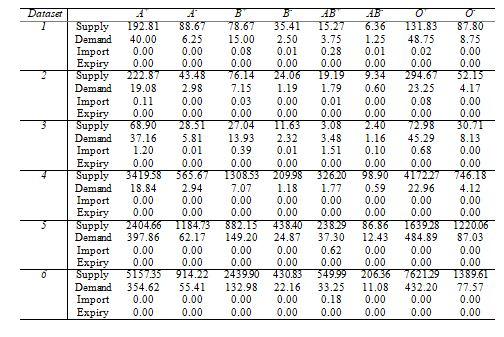
\includegraphics[width=0.8\textwidth, center]{Images/Tab8.JPG}
\\
\\
In Table 8 and Figs. 3 to 8, the results indicate that the hybrid SOS algorithm coupled with the blood management policy achieved good results in terms of having very low importation levels and no form of expiry across any of the datasets. The results also show that stock-piling occurs at early period within the time frame which supports low importation levels, but opens the system to possible expiry, however this phenomenon did not occur due to the 30 shelf life of WB units as well as the FIFO issuing system. It would be unrealistic for any WB units not to be used within the 30-day time frame, unless demand was extremely low. As aforementioned, stock-piling is a phenomenon which can almost eradicate WB importation, depending on how fast this even occurs. For most datasets, stock-piling occurs at a relatively early period (excluding the case of dataset 4: which tested demand levels greater than supply levels). however, for much rarer blood types, stock-piling doesn’t occur as the levels are simply too low to start accumulation.
\\
\\
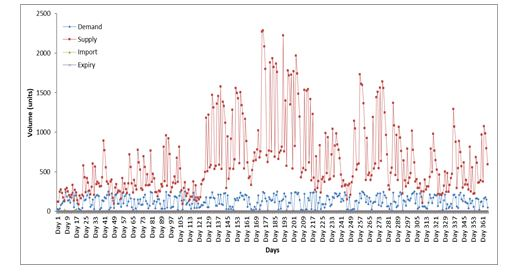
\includegraphics[width=0.8\textwidth, center]{Images/Fig3.JPG}
\begin {center}
Fig. 3: { SOS implementation of dataset 1 over a period of 365 days}
\end{center}\\
\\
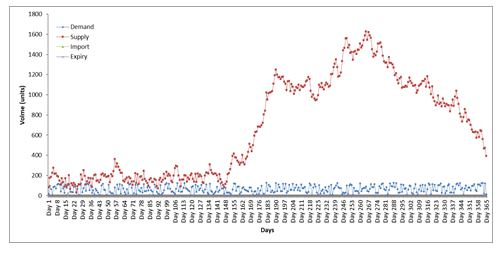
\includegraphics[width=0.75\textwidth, center]{Images/Fig4.JPG}
\begin {center}
Fig. 4: { SOS implementation of dataset 2 over a period of 365 days}

\end {center}

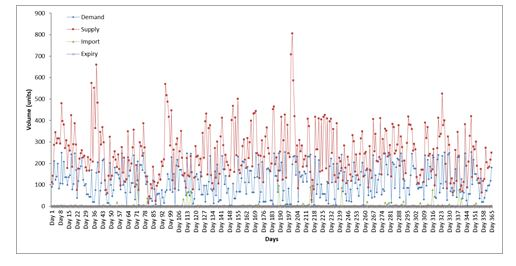
\includegraphics[width=0.75\textwidth, center]{Images/Fig5.JPG}
\begin {center}
Fig. 5: { SOS implementation of dataset 3 over a period of 365 days}
\break
\end {center}

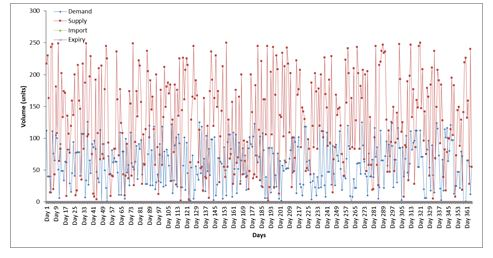
\includegraphics[width=0.75\textwidth, center]{Images/Fig6.JPG}
\begin {center}
Fig. 6: { SOS implementation of dataset 4 over a period of 365 days}

\end {center}

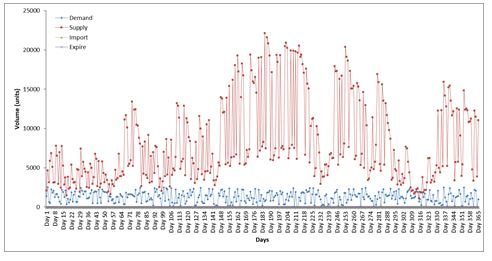
\includegraphics[width=0.75\textwidth, center]{Images/Fig7.JPG}
\begin {center}
Fig. 7: { SOS implementation of dataset 5 over a period of 365 days}

\end {center}


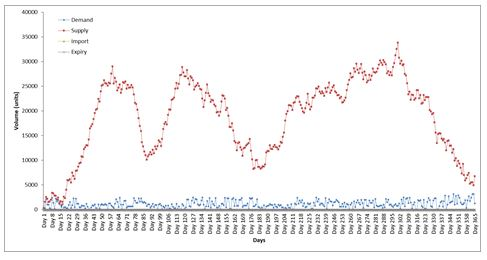
\includegraphics[width=0.75\textwidth, center]{Images/Fig8.JPG}
\begin {center}
Fig. 8: { SOS implementation of dataset 6 over a period of 365 days}

\end {center}
\\
\\
The studies conducted in [3], [4], [6], and [7] used constant percentage bounds ranging between 27-75\% in order to generate values for demand. These bounds were used across the entire testing range of 365 days. The current study allocates specific percentage ranges to each month with the aim of generating more accurate demand levels in accordance to the South African monthly schooling terms and public holidays. Ideally, the best source of generating demand percentage bounds would preferably be statistics based on actual demand for WB units within South Africa, however, these statistics was not available. For easier identification, “Demand (25\%-75\%)” represents demand generated using the constant percentage bounds between 25-75\% and “Demand (SAGV)” represents the SAGV for demand. The average demand generated using the Demand SAGV is lower due to the varying percentage ranges, each month is exposed to a very low percentage bound, which in turn reduces the overall average, unlike in the case of the constant percentage bounds (27\%-75\%), which has a constant percentage range. Figure 9 depicts the demand curvature for the SOS implementation for the two different percentage bound generations. Although the statistics used in generating these demands are stochastic, its provides some form of stability which can be improved upon and makes the current study replicable. Furthermore, the implementation of the Demand SAGV technique, shows prospect in reducing randomness in generating demand values which in turn provides more accurate results, specifically for the BAP, whose real-world datasets information are not publicly available.
\\
\\
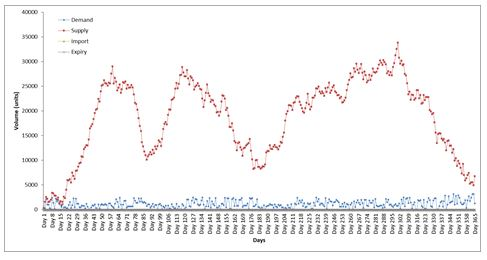
\includegraphics[width=0.75\textwidth, center]{Images/Fig8.JPG}
\begin {center}
Fig. 9: {Comparison between demand generations for SOS}

\end {center}\\

\subsection{Comparison with results from literature}
Few of the available BAP literature considered different metaheuristic algorithms for the BAP. Most of these studies followed similar problem formulation model with minor differences. In order to assess the performance of the SOS algorithm in relation to the BAP, the numerical results obtained by the SOS is compared with the results obtained from the related literatures. Due to the difference in style of data generation and experimental configurations, it was impossible to compare the results of the proposed algorithm with some of the existing literature results. However, the results presented in [2] and [6] are investigated for possible comparisons with the proposed SOS algorithm. Although each of the existing literature implemented a different metaheuristic algorithm, they both employed similar blood banking structures and assignment policies to solve the BAP. Therefore, the respective implemented algorithms that produced the best results are subsequently identified and compared with the proposed SOS algorithm. In Tables 9 and 10, the average number of importation (AI) and the percentage proportion of import (PI) are the two evaluation metrics used to compare SOS and other existing techniques. However, AI is determined based on the algorithm execution as objective function, while PI(\%) is calculated using the following equations.\\
\\
$PI(\%) = \[\frac{AI{_B}}{\sum{_{k=1}^8}. AI{_{B_{TOT}}}} . 100\]$ \tab[12cm](12)\\
\\
Where:\\
B: Represents a blood type\\
$B{_{Tot}}$: Represents all the blood types\\
\\
The first comparison is based on the work presented in [2], which implemented 7 datasets, but dataset 6 and 7 will only be examined as the time period lasted for 365 days and are identical to the time period of the datasets 1 and 5 used to implement the SOS algorithm presented in this paper. Moreover, the datasets 6 and 7 implemented in [2] used the same percentage bounds range of between 25-75\% for both demand and supply, but used an initial volume of 500 WB units in dataset 6 and 1000 units in dataset 7.  In addition to using similar dataset, they also implemented PSO algorithm to solve the BAP. These datasets could be compared to dataset 1 and 6 in the SOS study as they are similar with regards to parameter configurations. The results presented Table 9 show the average results obtained for the respective datasets, namely, 1, 5, 6, 7. Comparing the results from the two study, it can be seen that the PSO algorithm proposed in [2] produced much larger average solutions for these blood types with a total average of 1.8 WB unit import, whilst the SOS algorithm only recorded an average of 0.4 WB unit import. The drastic difference can be attributed to SOS utilising the previous days remaining of WB units, which was not considered in [2]. Furthermore, it was observed that the best algorithm for dataset 5 was the SOS algorithm, as it incurred no importation except for blood type AB+. The study in [2] displayed a total average of 5.46 WB units. Overall the comparison between these two studies has justified that the act of using the previous day’s remaining WB units to treat patients greatly reduces the levels of importation.\\
\\
\begin {center}
Table 9: {Comparison of average importation results obtained in [2] with SOS}

\end {center}
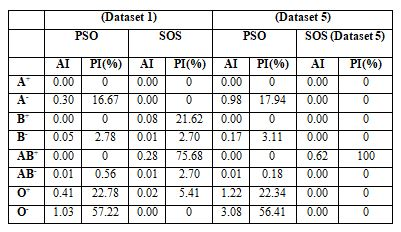
\includegraphics[width=0.6\textwidth, center]{Images/CompTab.JPG}
\\
\\
The second comparison is with the study presented in [6]. The dataset 1 in [6] used an initial WB unit volume of 500 units and percentage bounds between 25-75\%, which can be compared to the current study’s dataset 1. Likewise, dataset 3 used a larger initial volume of WB units (2000 units) with the same percentage bounds as dataset 1, and can therefore be compared to dataset 5 of the current study. The averages results obtained in [6] were calculated over a period of 90 days with blood type O+ and O- recording the largest average importation levels. The SOS implementation in this study out-performed the HC algorithm, but did experience higher averages for blood types B+ and AB+ as compared to the results in [6]. Furthermore, the dataset 3 in [6] used an initial WB unit volume of 2000, but still produced much larger averages as compared to the SOS algorithm in this study. In [6], the blood types AB+ and AB- results recorded no form of importation, whilst the proposed SOS algorithm incurred imports for blood type AB+. This could imply that the HC algorithm performs well only for types AB+ and AB- when exposed to larger WB unit volumes.
\\
\\
\begin {center}
Table 10: {Comparison of average importation results obtained in [6] with SOS}

\end {center}
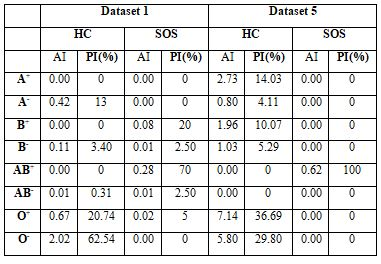
\includegraphics[width=0.6\textwidth, center]{Images/CompTab2.JPG}\\
\\
In summary, an important aspect of this study for the BAP relates to the random generation of demand values. As mentioned earlier in section 2, this study incorporates values which conformed to the South African public holidays and schooling terms (which in turn points at South African social behaviour). In Fig. 9, the graphs illustrate trends in demand levels. When using a fixed percentage bounds (25-75\%), the demand levels are stochastic which should not be the case, as the demand for WB units should have higher levels during certain periods in a year. The introduction of generating demand using unique percentage bounds allocated to each month manage to successfully give a more accurate reading for demand levels. Due to the fixed percentage bounds being constant throughout the time period, and the SAGV demand generation having much lower demand values at certain periods, the overall average of the fixed percentage approach is much higher in comparison to the SAGV approach. Even though real-world data could not be located, the ideology can be expanded upon in future literature with blood management problems, or any other perishable inventory problem.
\section{Results and Future Directions}
This paper presents a hybrid metaheuristic algorithm, which combines symbiotic organism search algorithm with a blood assignment heuristic method to solve the BAP. Based on the results discussed in this paper, it is obvious that the hybrid SOS implementation successfully achieved the objective function of the BAP. The implementation had very low amounts of importation, and no form of expiration when subjected to any of the datasets. The low importation levels can be attributed to the effects of using the bottom-up technique which promoted the use of compatible blood types, and the lack of expiry can be linked to the FIFO issuing system. Using dataset 1 as a control, it was possible to establish how effective the demand generation was in relation to using SAGV. Dataset 2 experienced a 42.5\% overall decrease in the total levels for importation, whilst dataset 5 and 6 used the same percentage bounds as dataset 1 and 2, but had a much larger initial volume of WB units. Dataset 6 (which used SAGV for generating demand), also experienced a lower importation level by 44\%. In relation to dataset 1 and 2 in terms of demand generation, dataset 2 used the SAGV approach, and experienced a 52\% decrease in overall demand, whilst supply increased by 14\%, which was to be expected due to the act of stock-piling. Reflecting upon the existing PSO algorithm, in comparison to dataset 1 (which followed the same data generation guidelines), the hybrid SOS algorithm performed better with a 73\% decrease in total importation. Likewise, the SAGV approach also incurred a far lower importation rate of 84\%. However, it must be noted that the existing PSO implementation was conducted over 90 days’ time frame. It is difficult to judge other related work, as the time period in which the algorithms were conducted did not follow the same number of days as in this study, or the dataset generation used different initial WB unit volumes. 
\\
\\
Future work can improve upon the generation of demand values by utilising more accurate statistics from a population. The use of more assumptions can be introduced to try and alter the mathematical model, as well as using real life data rather than randomly generated datasets. The following study has tried to bridge the gap between previous literatures by means of exploring new metaheuristic algorithm as well as try to contribute towards the study of blood management, as well as other inventory problems relating to perishable items. 
\\
\\
\textbf{References}\\
\\
1.	Hesse S, Coullard C, Daskin M, Hurter A. A case study in platelet inventory management. InProceedings of the 6th Industrial Engineering Research Conference. Atlanta: Institute of Industrial Engineers 1997 (pp. 801-6).\\
2.	Olusanya MO, Arasomwan MA, Adewumi AO. Particle swarm optimization algorithm for optimizing assignment of blood in blood banking system. Computational and mathematical methods in medicine. 2015;2015.\\
3.	Reid ME, Lomas-Francis C, Olsson ML. The blood group antigen factsbook. Academic press; 2012 Nov 7.\\
4.	Charpin JP, Adewumi AO. Optimal assignment of blood in a blood banking System. Tech. Rep., Mathematics in Industry Study Group (MISG); 2011. \\
5.	Baş S, Carello G, Lanzarone E, Ocak Z, Yalçındağ S. Management of blood donation system: literature review and research perspectives. InHealth Care Systems Engineering for Scientists and Practitioners 2016 (pp. 121-132). Springer, Cham.\\
6.	Adewumi A, Budlender N, Olusanya M. Optimizing the assignment of blood in a blood banking system: some initial results. InEvolutionary Computation (CEC), 2012 IEEE Congress on 2012 Jun 10 (pp. 1-6). IEEE.\\
7.	Igwe K, Olusanya M, Adewumi A. On the performance of GRASP and dynamic programming for the blood assignment problem. InGHTC 2013 Oct 20 (pp. 221-225).\\
8.	Statistics South Africa. Mid-year population estimates. Statistics South Africa; 2017, pp 1:\\ https://www.statssa.gov.za/publications/P0302/P03022016.pdf \\
9.	South African National Blood Service, What’s your type, http://www.sanbs.org.za, [Accessed on 17/05/2018].\\
10.	Lewis RO. Independent verification and validation: A life cycle engineering process for quality software. John Wiley & Sons; 1992.\\
11.	https://www.news24.com/SouthAfrica/News/easter-road-death-toll-up-by-14-from-last-year-20180417, visited: [04-06-2018]\\
12.	http://www.schoolterms.co.za/2018.html, [Accessed on 04-06-2018]\\
13.	Cheng MY, Prayogo D. Symbiotic organisms search: a new metaheuristic optimization algorithm. Computers & Structures. 2014 Jul 15;139:98-112.\\
14.	Cheng MY, Prayogo D, Tran DH. Optimizing multiple-resources leveling in multiple projects using discrete symbiotic organisms search. Journal of Computing in Civil Engineering. 2015 Jun 16;30(3):04015036.\\
15.	Cheng, M. Y, Prayogo, D. Symbiotic organism search: A new metaheuristic optimization. Computers and Structures, 139:98-112, 2014.\\
16.	Ezugwu, A.E.S., Adewumi, A.O. and Frîncu, M.E., 2017. Simulated annealing based symbiotic organisms search optimization algorithm for traveling salesman problem. Expert Systems with Applications, 77, pp.189-210.\\
17.	Tran, D.H., Cheng, M.Y. and Prayogo, D., 2016. A novel Multiple Objective Symbiotic Organisms Search (MOSOS) for time–cost–labor utilization tradeoff problem. Knowledge-Based Systems, 94, pp.132-145.\\
18.	Cheng, M.Y., Prayogo, D. and Tran, D.H., 2015. Optimizing multiple-resources leveling in multiple projects using discrete symbiotic organisms search. Journal of Computing in Civil Engineering, 30(3), p.04015036.\\
19.	Ezugwu, A.E., Adeleke, O.J. and Viriri, S., 2018. Symbiotic organisms search algorithm for the unrelated parallel machines scheduling with sequence-dependent setup times. PloS one, 13(7), p.e0200030.\\

\end{document}
